% Created by tikzDevice version 0.12 on 2019-05-07 15:15:52
% !TEX encoding = UTF-8 Unicode
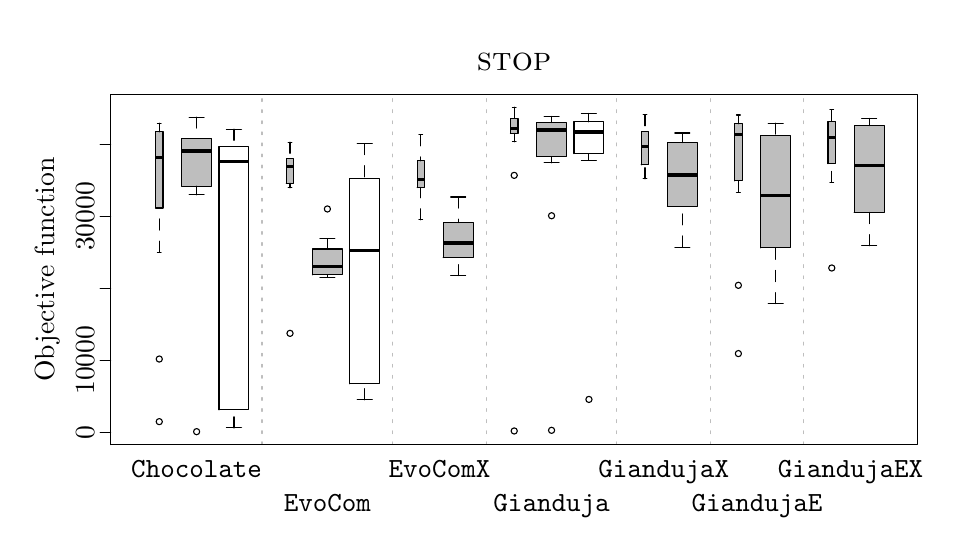
\begin{tikzpicture}[x=1pt,y=1pt]
\definecolor{fillColor}{RGB}{255,255,255}
\path[use as bounding box,fill=fillColor,fill opacity=0.00] (0,0) rectangle (325.21,180.67);
\begin{scope}
\path[clip] ( 30.00, 30.00) rectangle (321.61,156.67);
\definecolor{fillColor}{RGB}{190,190,190}

\path[fill=fillColor] ( 46.20,115.52) --
	( 48.90,115.52) --
	( 48.90,143.04) --
	( 46.20,143.04) --
	cycle;
\definecolor{drawColor}{RGB}{0,0,0}

\path[draw=drawColor,line width= 1.2pt,line join=round] ( 46.20,133.75) -- ( 48.90,133.75);

\path[draw=drawColor,line width= 0.4pt,dash pattern=on 4pt off 4pt ,line join=round,line cap=round] ( 47.55, 99.56) -- ( 47.55,115.52);

\path[draw=drawColor,line width= 0.4pt,dash pattern=on 4pt off 4pt ,line join=round,line cap=round] ( 47.55,146.15) -- ( 47.55,143.04);

\path[draw=drawColor,line width= 0.4pt,line join=round,line cap=round] ( 46.88, 99.56) -- ( 48.23, 99.56);

\path[draw=drawColor,line width= 0.4pt,line join=round,line cap=round] ( 46.88,146.15) -- ( 48.23,146.15);

\path[draw=drawColor,line width= 0.4pt,line join=round,line cap=round] ( 46.20,115.52) --
	( 48.90,115.52) --
	( 48.90,143.04) --
	( 46.20,143.04) --
	( 46.20,115.52);

\path[draw=drawColor,line width= 0.4pt,line join=round,line cap=round] ( 47.55, 60.93) circle (  1.12);

\path[draw=drawColor,line width= 0.4pt,line join=round,line cap=round] ( 47.55, 38.31) circle (  1.12);

\path[fill=fillColor] ( 55.65,123.37) --
	( 66.45,123.37) --
	( 66.45,140.78) --
	( 55.65,140.78) --
	cycle;

\path[draw=drawColor,line width= 1.2pt,line join=round] ( 55.65,136.16) -- ( 66.45,136.16);

\path[draw=drawColor,line width= 0.4pt,dash pattern=on 4pt off 4pt ,line join=round,line cap=round] ( 61.05,120.29) -- ( 61.05,123.37);

\path[draw=drawColor,line width= 0.4pt,dash pattern=on 4pt off 4pt ,line join=round,line cap=round] ( 61.05,148.35) -- ( 61.05,140.78);

\path[draw=drawColor,line width= 0.4pt,line join=round,line cap=round] ( 58.35,120.29) -- ( 63.75,120.29);

\path[draw=drawColor,line width= 0.4pt,line join=round,line cap=round] ( 58.35,148.35) -- ( 63.75,148.35);

\path[draw=drawColor,line width= 0.4pt,line join=round,line cap=round] ( 55.65,123.37) --
	( 66.45,123.37) --
	( 66.45,140.78) --
	( 55.65,140.78) --
	( 55.65,123.37);

\path[draw=drawColor,line width= 0.4pt,line join=round,line cap=round] ( 61.05, 34.69) circle (  1.12);
\definecolor{fillColor}{RGB}{255,255,255}

\path[fill=fillColor] ( 69.15, 42.59) --
	( 79.95, 42.59) --
	( 79.95,137.61) --
	( 69.15,137.61) --
	cycle;

\path[draw=drawColor,line width= 1.2pt,line join=round] ( 69.15,132.27) -- ( 79.95,132.27);

\path[draw=drawColor,line width= 0.4pt,dash pattern=on 4pt off 4pt ,line join=round,line cap=round] ( 74.55, 36.05) -- ( 74.55, 42.59);

\path[draw=drawColor,line width= 0.4pt,dash pattern=on 4pt off 4pt ,line join=round,line cap=round] ( 74.55,143.97) -- ( 74.55,137.61);

\path[draw=drawColor,line width= 0.4pt,line join=round,line cap=round] ( 71.85, 36.05) -- ( 77.25, 36.05);

\path[draw=drawColor,line width= 0.4pt,line join=round,line cap=round] ( 71.85,143.97) -- ( 77.25,143.97);

\path[draw=drawColor,line width= 0.4pt,line join=round,line cap=round] ( 69.15, 42.59) --
	( 79.95, 42.59) --
	( 79.95,137.61) --
	( 69.15,137.61) --
	( 69.15, 42.59);
\definecolor{fillColor}{RGB}{190,190,190}

\path[fill=fillColor] ( 93.45,124.44) --
	( 96.15,124.44) --
	( 96.15,133.29) --
	( 93.45,133.29) --
	cycle;

\path[draw=drawColor,line width= 1.2pt,line join=round] ( 93.45,130.43) -- ( 96.15,130.43);

\path[draw=drawColor,line width= 0.4pt,dash pattern=on 4pt off 4pt ,line join=round,line cap=round] ( 94.80,122.81) -- ( 94.80,124.44);

\path[draw=drawColor,line width= 0.4pt,dash pattern=on 4pt off 4pt ,line join=round,line cap=round] ( 94.80,139.29) -- ( 94.80,133.29);

\path[draw=drawColor,line width= 0.4pt,line join=round,line cap=round] ( 94.13,122.81) -- ( 95.48,122.81);

\path[draw=drawColor,line width= 0.4pt,line join=round,line cap=round] ( 94.13,139.29) -- ( 95.48,139.29);

\path[draw=drawColor,line width= 0.4pt,line join=round,line cap=round] ( 93.45,124.44) --
	( 96.15,124.44) --
	( 96.15,133.29) --
	( 93.45,133.29) --
	( 93.45,124.44);

\path[draw=drawColor,line width= 0.4pt,line join=round,line cap=round] ( 94.80, 70.21) circle (  1.12);

\path[fill=fillColor] (102.90, 91.38) --
	(113.70, 91.38) --
	(113.70,100.69) --
	(102.90,100.69) --
	cycle;

\path[draw=drawColor,line width= 1.2pt,line join=round] (102.90, 94.39) -- (113.70, 94.39);

\path[draw=drawColor,line width= 0.4pt,dash pattern=on 4pt off 4pt ,line join=round,line cap=round] (108.30, 90.45) -- (108.30, 91.38);

\path[draw=drawColor,line width= 0.4pt,dash pattern=on 4pt off 4pt ,line join=round,line cap=round] (108.30,104.35) -- (108.30,100.69);

\path[draw=drawColor,line width= 0.4pt,line join=round,line cap=round] (105.60, 90.45) -- (111.00, 90.45);

\path[draw=drawColor,line width= 0.4pt,line join=round,line cap=round] (105.60,104.35) -- (111.00,104.35);

\path[draw=drawColor,line width= 0.4pt,line join=round,line cap=round] (102.90, 91.38) --
	(113.70, 91.38) --
	(113.70,100.69) --
	(102.90,100.69) --
	(102.90, 91.38);

\path[draw=drawColor,line width= 0.4pt,line join=round,line cap=round] (108.30,115.16) circle (  1.12);
\definecolor{fillColor}{RGB}{255,255,255}

\path[fill=fillColor] (116.40, 52.01) --
	(127.20, 52.01) --
	(127.20,126.18) --
	(116.40,126.18) --
	cycle;

\path[draw=drawColor,line width= 1.2pt,line join=round] (116.40,100.25) -- (127.20,100.25);

\path[draw=drawColor,line width= 0.4pt,dash pattern=on 4pt off 4pt ,line join=round,line cap=round] (121.80, 46.19) -- (121.80, 52.01);

\path[draw=drawColor,line width= 0.4pt,dash pattern=on 4pt off 4pt ,line join=round,line cap=round] (121.80,138.78) -- (121.80,126.18);

\path[draw=drawColor,line width= 0.4pt,line join=round,line cap=round] (119.10, 46.19) -- (124.50, 46.19);

\path[draw=drawColor,line width= 0.4pt,line join=round,line cap=round] (119.10,138.78) -- (124.50,138.78);

\path[draw=drawColor,line width= 0.4pt,line join=round,line cap=round] (116.40, 52.01) --
	(127.20, 52.01) --
	(127.20,126.18) --
	(116.40,126.18) --
	(116.40, 52.01);
\definecolor{fillColor}{RGB}{190,190,190}

\path[fill=fillColor] (140.71,122.88) --
	(143.41,122.88) --
	(143.41,132.53) --
	(140.71,132.53) --
	cycle;

\path[draw=drawColor,line width= 1.2pt,line join=round] (140.71,125.90) -- (143.41,125.90);

\path[draw=drawColor,line width= 0.4pt,dash pattern=on 4pt off 4pt ,line join=round,line cap=round] (142.06,111.22) -- (142.06,122.88);

\path[draw=drawColor,line width= 0.4pt,dash pattern=on 4pt off 4pt ,line join=round,line cap=round] (142.06,142.00) -- (142.06,132.53);

\path[draw=drawColor,line width= 0.4pt,line join=round,line cap=round] (141.38,111.22) -- (142.73,111.22);

\path[draw=drawColor,line width= 0.4pt,line join=round,line cap=round] (141.38,142.00) -- (142.73,142.00);

\path[draw=drawColor,line width= 0.4pt,line join=round,line cap=round] (140.71,122.88) --
	(143.41,122.88) --
	(143.41,132.53) --
	(140.71,132.53) --
	(140.71,122.88);

\path[fill=fillColor] (150.16, 97.62) --
	(160.96, 97.62) --
	(160.96,110.26) --
	(150.16,110.26) --
	cycle;

\path[draw=drawColor,line width= 1.2pt,line join=round] (150.16,102.91) -- (160.96,102.91);

\path[draw=drawColor,line width= 0.4pt,dash pattern=on 4pt off 4pt ,line join=round,line cap=round] (155.56, 91.07) -- (155.56, 97.62);

\path[draw=drawColor,line width= 0.4pt,dash pattern=on 4pt off 4pt ,line join=round,line cap=round] (155.56,119.49) -- (155.56,110.26);

\path[draw=drawColor,line width= 0.4pt,line join=round,line cap=round] (152.86, 91.07) -- (158.26, 91.07);

\path[draw=drawColor,line width= 0.4pt,line join=round,line cap=round] (152.86,119.49) -- (158.26,119.49);

\path[draw=drawColor,line width= 0.4pt,line join=round,line cap=round] (150.16, 97.62) --
	(160.96, 97.62) --
	(160.96,110.26) --
	(150.16,110.26) --
	(150.16, 97.62);

\path[fill=fillColor] (174.46,142.49) --
	(177.16,142.49) --
	(177.16,148.00) --
	(174.46,148.00) --
	cycle;

\path[draw=drawColor,line width= 1.2pt,line join=round] (174.46,144.28) -- (177.16,144.28);

\path[draw=drawColor,line width= 0.4pt,dash pattern=on 4pt off 4pt ,line join=round,line cap=round] (175.81,139.41) -- (175.81,142.49);

\path[draw=drawColor,line width= 0.4pt,dash pattern=on 4pt off 4pt ,line join=round,line cap=round] (175.81,151.98) -- (175.81,148.00);

\path[draw=drawColor,line width= 0.4pt,line join=round,line cap=round] (175.13,139.41) -- (176.48,139.41);

\path[draw=drawColor,line width= 0.4pt,line join=round,line cap=round] (175.13,151.98) -- (176.48,151.98);

\path[draw=drawColor,line width= 0.4pt,line join=round,line cap=round] (174.46,142.49) --
	(177.16,142.49) --
	(177.16,148.00) --
	(174.46,148.00) --
	(174.46,142.49);

\path[draw=drawColor,line width= 0.4pt,line join=round,line cap=round] (175.81,127.30) circle (  1.12);

\path[draw=drawColor,line width= 0.4pt,line join=round,line cap=round] (175.81, 34.94) circle (  1.12);

\path[fill=fillColor] (183.91,134.06) --
	(194.71,134.06) --
	(194.71,146.38) --
	(183.91,146.38) --
	cycle;

\path[draw=drawColor,line width= 1.2pt,line join=round] (183.91,143.66) -- (194.71,143.66);

\path[draw=drawColor,line width= 0.4pt,dash pattern=on 4pt off 4pt ,line join=round,line cap=round] (189.31,131.84) -- (189.31,134.06);

\path[draw=drawColor,line width= 0.4pt,dash pattern=on 4pt off 4pt ,line join=round,line cap=round] (189.31,148.57) -- (189.31,146.38);

\path[draw=drawColor,line width= 0.4pt,line join=round,line cap=round] (186.61,131.84) -- (192.01,131.84);

\path[draw=drawColor,line width= 0.4pt,line join=round,line cap=round] (186.61,148.57) -- (192.01,148.57);

\path[draw=drawColor,line width= 0.4pt,line join=round,line cap=round] (183.91,134.06) --
	(194.71,134.06) --
	(194.71,146.38) --
	(183.91,146.38) --
	(183.91,134.06);

\path[draw=drawColor,line width= 0.4pt,line join=round,line cap=round] (189.31,112.71) circle (  1.12);

\path[draw=drawColor,line width= 0.4pt,line join=round,line cap=round] (189.31, 35.17) circle (  1.12);
\definecolor{fillColor}{RGB}{255,255,255}

\path[fill=fillColor] (197.41,135.17) --
	(208.21,135.17) --
	(208.21,146.65) --
	(197.41,146.65) --
	cycle;

\path[draw=drawColor,line width= 1.2pt,line join=round] (197.41,142.93) -- (208.21,142.93);

\path[draw=drawColor,line width= 0.4pt,dash pattern=on 4pt off 4pt ,line join=round,line cap=round] (202.81,132.77) -- (202.81,135.17);

\path[draw=drawColor,line width= 0.4pt,dash pattern=on 4pt off 4pt ,line join=round,line cap=round] (202.81,149.64) -- (202.81,146.65);

\path[draw=drawColor,line width= 0.4pt,line join=round,line cap=round] (200.11,132.77) -- (205.51,132.77);

\path[draw=drawColor,line width= 0.4pt,line join=round,line cap=round] (200.11,149.64) -- (205.51,149.64);

\path[draw=drawColor,line width= 0.4pt,line join=round,line cap=round] (197.41,135.17) --
	(208.21,135.17) --
	(208.21,146.65) --
	(197.41,146.65) --
	(197.41,135.17);

\path[draw=drawColor,line width= 0.4pt,line join=round,line cap=round] (202.81, 46.34) circle (  1.12);
\definecolor{fillColor}{RGB}{190,190,190}

\path[fill=fillColor] (221.71,131.14) --
	(224.41,131.14) --
	(224.41,143.27) --
	(221.71,143.27) --
	cycle;

\path[draw=drawColor,line width= 1.2pt,line join=round] (221.71,137.85) -- (224.41,137.85);

\path[draw=drawColor,line width= 0.4pt,dash pattern=on 4pt off 4pt ,line join=round,line cap=round] (223.06,126.08) -- (223.06,131.14);

\path[draw=drawColor,line width= 0.4pt,dash pattern=on 4pt off 4pt ,line join=round,line cap=round] (223.06,149.21) -- (223.06,143.27);

\path[draw=drawColor,line width= 0.4pt,line join=round,line cap=round] (222.38,126.08) -- (223.73,126.08);

\path[draw=drawColor,line width= 0.4pt,line join=round,line cap=round] (222.38,149.21) -- (223.73,149.21);

\path[draw=drawColor,line width= 0.4pt,line join=round,line cap=round] (221.71,131.14) --
	(224.41,131.14) --
	(224.41,143.27) --
	(221.71,143.27) --
	(221.71,131.14);

\path[fill=fillColor] (231.16,116.13) --
	(241.96,116.13) --
	(241.96,139.14) --
	(231.16,139.14) --
	cycle;

\path[draw=drawColor,line width= 1.2pt,line join=round] (231.16,127.45) -- (241.96,127.45);

\path[draw=drawColor,line width= 0.4pt,dash pattern=on 4pt off 4pt ,line join=round,line cap=round] (236.56,101.39) -- (236.56,116.13);

\path[draw=drawColor,line width= 0.4pt,dash pattern=on 4pt off 4pt ,line join=round,line cap=round] (236.56,142.59) -- (236.56,139.14);

\path[draw=drawColor,line width= 0.4pt,line join=round,line cap=round] (233.86,101.39) -- (239.26,101.39);

\path[draw=drawColor,line width= 0.4pt,line join=round,line cap=round] (233.86,142.59) -- (239.26,142.59);

\path[draw=drawColor,line width= 0.4pt,line join=round,line cap=round] (231.16,116.13) --
	(241.96,116.13) --
	(241.96,139.14) --
	(231.16,139.14) --
	(231.16,116.13);

\path[fill=fillColor] (255.46,125.29) --
	(258.16,125.29) --
	(258.16,145.96) --
	(255.46,145.96) --
	cycle;

\path[draw=drawColor,line width= 1.2pt,line join=round] (255.46,141.97) -- (258.16,141.97);

\path[draw=drawColor,line width= 0.4pt,dash pattern=on 4pt off 4pt ,line join=round,line cap=round] (256.81,121.22) -- (256.81,125.29);

\path[draw=drawColor,line width= 0.4pt,dash pattern=on 4pt off 4pt ,line join=round,line cap=round] (256.81,149.11) -- (256.81,145.96);

\path[draw=drawColor,line width= 0.4pt,line join=round,line cap=round] (256.14,121.22) -- (257.49,121.22);

\path[draw=drawColor,line width= 0.4pt,line join=round,line cap=round] (256.14,149.11) -- (257.49,149.11);

\path[draw=drawColor,line width= 0.4pt,line join=round,line cap=round] (255.46,125.29) --
	(258.16,125.29) --
	(258.16,145.96) --
	(255.46,145.96) --
	(255.46,125.29);

\path[draw=drawColor,line width= 0.4pt,line join=round,line cap=round] (256.81, 62.90) circle (  1.12);

\path[draw=drawColor,line width= 0.4pt,line join=round,line cap=round] (256.81, 87.57) circle (  1.12);

\path[fill=fillColor] (264.91,101.10) --
	(275.71,101.10) --
	(275.71,141.66) --
	(264.91,141.66) --
	cycle;

\path[draw=drawColor,line width= 1.2pt,line join=round] (264.91,120.10) -- (275.71,120.10);

\path[draw=drawColor,line width= 0.4pt,dash pattern=on 4pt off 4pt ,line join=round,line cap=round] (270.31, 80.93) -- (270.31,101.10);

\path[draw=drawColor,line width= 0.4pt,dash pattern=on 4pt off 4pt ,line join=round,line cap=round] (270.31,146.18) -- (270.31,141.66);

\path[draw=drawColor,line width= 0.4pt,line join=round,line cap=round] (267.61, 80.93) -- (273.01, 80.93);

\path[draw=drawColor,line width= 0.4pt,line join=round,line cap=round] (267.61,146.18) -- (273.01,146.18);

\path[draw=drawColor,line width= 0.4pt,line join=round,line cap=round] (264.91,101.10) --
	(275.71,101.10) --
	(275.71,141.66) --
	(264.91,141.66) --
	(264.91,101.10);

\path[fill=fillColor] (289.21,131.52) --
	(291.91,131.52) --
	(291.91,146.89) --
	(289.21,146.89) --
	cycle;

\path[draw=drawColor,line width= 1.2pt,line join=round] (289.21,141.09) -- (291.91,141.09);

\path[draw=drawColor,line width= 0.4pt,dash pattern=on 4pt off 4pt ,line join=round,line cap=round] (290.56,124.76) -- (290.56,131.52);

\path[draw=drawColor,line width= 0.4pt,dash pattern=on 4pt off 4pt ,line join=round,line cap=round] (290.56,151.00) -- (290.56,146.89);

\path[draw=drawColor,line width= 0.4pt,line join=round,line cap=round] (289.89,124.76) -- (291.24,124.76);

\path[draw=drawColor,line width= 0.4pt,line join=round,line cap=round] (289.89,151.00) -- (291.24,151.00);

\path[draw=drawColor,line width= 0.4pt,line join=round,line cap=round] (289.21,131.52) --
	(291.91,131.52) --
	(291.91,146.89) --
	(289.21,146.89) --
	(289.21,131.52);

\path[draw=drawColor,line width= 0.4pt,line join=round,line cap=round] (290.56, 93.83) circle (  1.12);

\path[fill=fillColor] (298.66,113.99) --
	(309.46,113.99) --
	(309.46,145.32) --
	(298.66,145.32) --
	cycle;

\path[draw=drawColor,line width= 1.2pt,line join=round] (298.66,130.93) -- (309.46,130.93);

\path[draw=drawColor,line width= 0.4pt,dash pattern=on 4pt off 4pt ,line join=round,line cap=round] (304.06,101.88) -- (304.06,113.99);

\path[draw=drawColor,line width= 0.4pt,dash pattern=on 4pt off 4pt ,line join=round,line cap=round] (304.06,147.87) -- (304.06,145.32);

\path[draw=drawColor,line width= 0.4pt,line join=round,line cap=round] (301.36,101.88) -- (306.76,101.88);

\path[draw=drawColor,line width= 0.4pt,line join=round,line cap=round] (301.36,147.87) -- (306.76,147.87);

\path[draw=drawColor,line width= 0.4pt,line join=round,line cap=round] (298.66,113.99) --
	(309.46,113.99) --
	(309.46,145.32) --
	(298.66,145.32) --
	(298.66,113.99);
\definecolor{drawColor}{RGB}{190,190,190}

\path[draw=drawColor,line width= 0.4pt,dash pattern=on 1pt off 3pt ,line join=round,line cap=round] ( 84.68, 30.00) -- ( 84.68,156.67);

\path[draw=drawColor,line width= 0.4pt,dash pattern=on 1pt off 3pt ,line join=round,line cap=round] (131.93, 30.00) -- (131.93,156.67);

\path[draw=drawColor,line width= 0.4pt,dash pattern=on 1pt off 3pt ,line join=round,line cap=round] (165.68, 30.00) -- (165.68,156.67);

\path[draw=drawColor,line width= 0.4pt,dash pattern=on 1pt off 3pt ,line join=round,line cap=round] (212.93, 30.00) -- (212.93,156.67);

\path[draw=drawColor,line width= 0.4pt,dash pattern=on 1pt off 3pt ,line join=round,line cap=round] (246.69, 30.00) -- (246.69,156.67);

\path[draw=drawColor,line width= 0.4pt,dash pattern=on 1pt off 3pt ,line join=round,line cap=round] (280.44, 30.00) -- (280.44,156.67);
\end{scope}
\begin{scope}
\path[clip] (  0.00,  0.00) rectangle (325.21,180.67);
\definecolor{drawColor}{RGB}{0,0,0}

\node[text=drawColor,anchor=base,inner sep=0pt, outer sep=0pt, scale=  1.00] at ( 61.05, 18.00) {\texttt{Chocolate}};

\node[text=drawColor,anchor=base,inner sep=0pt, outer sep=0pt, scale=  1.00] at (148.81, 18.00) {\texttt{EvoComX}};

\node[text=drawColor,anchor=base,inner sep=0pt, outer sep=0pt, scale=  1.00] at (229.81, 18.00) {\texttt{GiandujaX}};

\node[text=drawColor,anchor=base,inner sep=0pt, outer sep=0pt, scale=  1.00] at (297.31, 18.00) {\texttt{GiandujaEX}};

\node[text=drawColor,anchor=base,inner sep=0pt, outer sep=0pt, scale=  1.00] at (108.30,  6.00) {\texttt{EvoCom}};

\node[text=drawColor,anchor=base,inner sep=0pt, outer sep=0pt, scale=  1.00] at (189.31,  6.00) {\texttt{Gianduja}};

\node[text=drawColor,anchor=base,inner sep=0pt, outer sep=0pt, scale=  1.00] at (263.56,  6.00) {\texttt{GiandujaE}};
\end{scope}
\begin{scope}
\path[clip] (  0.00,  0.00) rectangle (325.21,180.67);
\definecolor{drawColor}{RGB}{0,0,0}

\node[text=drawColor,anchor=base,inner sep=0pt, outer sep=0pt, scale=  1.20] at (175.81,165.07) {\textsc{stop}};

\node[text=drawColor,rotate= 90.00,anchor=base,inner sep=0pt, outer sep=0pt, scale=  1.00] at (  9.60, 93.34) {Objective function};
\end{scope}
\begin{scope}
\path[clip] (  0.00,  0.00) rectangle (325.21,180.67);
\definecolor{drawColor}{RGB}{0,0,0}

\path[draw=drawColor,line width= 0.4pt,line join=round,line cap=round] ( 30.00, 34.53) -- ( 30.00,138.51);

\path[draw=drawColor,line width= 0.4pt,line join=round,line cap=round] ( 30.00, 34.53) -- ( 26.20, 34.53);

\path[draw=drawColor,line width= 0.4pt,line join=round,line cap=round] ( 30.00, 60.52) -- ( 26.20, 60.52);

\path[draw=drawColor,line width= 0.4pt,line join=round,line cap=round] ( 30.00, 86.52) -- ( 26.20, 86.52);

\path[draw=drawColor,line width= 0.4pt,line join=round,line cap=round] ( 30.00,112.51) -- ( 26.20,112.51);

\path[draw=drawColor,line width= 0.4pt,line join=round,line cap=round] ( 30.00,138.51) -- ( 26.20,138.51);

\node[text=drawColor,rotate= 90.00,anchor=base,inner sep=0pt, outer sep=0pt, scale=  1.00] at ( 24.00, 34.53) {0};

\node[text=drawColor,rotate= 90.00,anchor=base,inner sep=0pt, outer sep=0pt, scale=  1.00] at ( 24.00, 60.52) {10000};

\node[text=drawColor,rotate= 90.00,anchor=base,inner sep=0pt, outer sep=0pt, scale=  1.00] at ( 24.00,112.51) {30000};

\path[draw=drawColor,line width= 0.4pt,line join=round,line cap=round] ( 30.00, 30.00) --
	(321.61, 30.00) --
	(321.61,156.67) --
	( 30.00,156.67) --
	( 30.00, 30.00);
\end{scope}
\end{tikzpicture}
